\chapter{The memory}
\label{ch:PGMEMORY}
The PostgreSQL memory at first sight looks simple if compared with the other RDBMS.
Actually the way PostgreSQL implements the memory manager to make the shared buffer 
capable to cache the data pages is sophisticated but incredibly simple to understand.

\section{The shared buffer}
The shared buffer is a shared segment allocated in the server's memory at cluster's startup. 
Its size is determined by the GUC parameter shared\_buffers and can be set only at the startup. 
The shared buffer is used to manage the data pages as seen in \ref{sec:CLUBACKEND}. When a page is loaded
in the shared buffer is called buffer. Shared segments in memory to speedup the data acces is common in the database universe. 
The drawback with this approach is that the memory is volatile and is completely lost if, for example, there is a power cut.

PostgreSQL aim to keep in memory only what is really important for the cluster's activity. In the era of the 
\textit{in memory databases} this maybe seems an obsolete concept. Unfortunately the sad truth is that the 
resources, are not infinite and sometimes the best line of action is a good compromise between cost and performance.
Before looking to the technical details we'll have a look to the history of the memory manager. 


\subsection{PostgreSQL 7.4, the LRU list}
Back in the old days PostgreSQL was quite rudimentary. The version 7.4 did not had tablespaces, it was 
without a mechanism to alert the DBA of the impending XID wraparound failure and the memory manager was a simple LRU buffer. 
Since then the algorithm evolved and became a very efficient system to cache the buffers. 

In PostgreSQL 7.4 the free space in the shared buffer was managed using a simple last recently used list implemented using a last recently used list.

There is a  list of pointers to the shared buffers. When a page is requested from the disk the buffer manager puts the buffer pointer into the first available position 
in the LRU list, switching the others pointers, if any, by one position. The last buffer in the list is evicted and then the pointer is removed. 

When a page is requested and is already present in the LRU LIST the corresponding pointer is moved on the top of the list. 
This simple approach works generally well. But because of the shared buffer is actually shared across the backends and the databases in the cluster, the different application logics
implemented for different databases can cause a suboptimal usage of the memory and an unnecessary disk IO. 

\subsubsection{The tale of the buffer}
I've found this interesting example years ago on Bruce Momjian's blog. The example explains very well how a 
minimal change in size can dramatically degrade the database performance.\newline

Our tale starts with a PostgreSQL 7.4 having a shared buffer sized to 1000 buffers. The page size is the default, 8192 bytes. 
We have in total \begin{math}8192 * 1000 = 8192000\end{math} available bytes to cache. 
Inside the data area we have a table without indices which is exactly 1000 pages. If we run a simple SELECT from the table,
PostgreSQL  will access the table with a sequential scan in order to get the buffers in memoy for reading. 
The sequential scan is a top to down operation. It starts from the first table's page and go on until reaches
the table's end. All the table's pages are read as the evaluation of the eventual WHERE condition is done in memory.

Initially the shared buffer is empty and the table's first page is put into the first slot of the LRU LIST.
The second page is then loaded causing the first page to shift a position in the LRU list. Then the third page is loaded as well causing another shift and so on.
When the table's read is finished the buffers are stored in the LRU list in reverse order. The first table's page is now allocated in the last LRU slot.

In this scenario, running again the SELECT is considerably faster. The table is again accessed in sequential scan but this time the first page is found in memory.
When accessed by the backend the page is moved in the first LRU slot causing the other buffers to shift and moving the second table's buffer into the empty slot of the LRU'S bottom.
Then the second page is accessed and moved on the top, causing the first page to shift on the second position and the third page to shift in the LRU bottom.
When the read is complete we'll found again the first page in the LRU's last slot. The perfect candidate for eviction.

If the table grows by one page the situation changes considerably. Running a SELECT with the shared buffer empty, loads again the entire table table in memory.
However, this time when the page 1001 is read the page allocated in the LRU's bottom is evicted.

A second run will cause another sequential scan on the table. The buffer manager will search in memory for the first page which was evicted by the page 1001.
The first page will then be loaded from the disk, causing the second page to be evicted from the memory. The second page is then loaded from disk causing the third page eviction and so on.

With the LRU adding an extra page in the table cause a dramatic performance degradation switching from 0\% IO to 100\% IO when accessing an already cached table.


\subsection{PostgreSQL 8.0, the 2q}
The revolutionary PostgreSQL 8.0 changed the game, switching to the algorithm called 2q (two queues) for the memory manager.\newline 

This algorithm uses three list of buffer pointers which are called cache directory blocks (CDB). The lists T1 and T2 point actual buffers. 
The list B1 is just a record of pages recently evicted from the shared buffer. 

\begin{figure}[H]
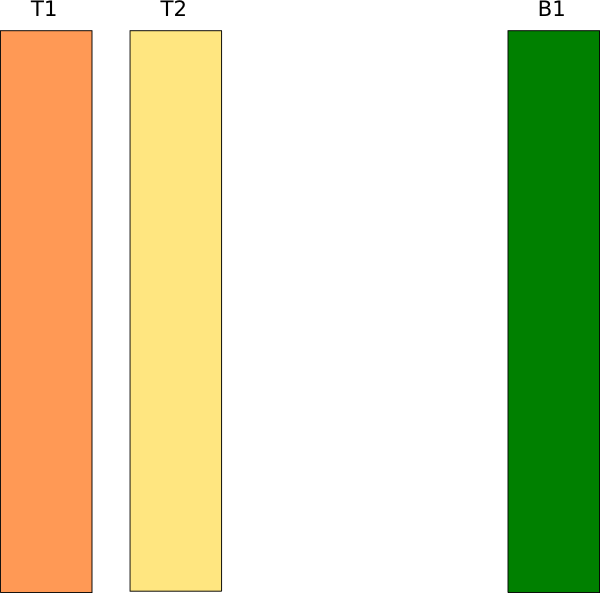
\includegraphics[scale=0.6]{images/shared_buffer_80.png}

\caption{PostgreSQL 8.0, CDB lists}

\end{figure}

The list T1 is used as LRU for the pages loaded from disk. The list T2 is used as LRU list for pages already cached 
and evicted from the list T1. The list B1 is a LRU list of pages recently evicted from the shared buffer.

When a new page is read from disk is put initially at the beginning of T1. All the CDB in T1 are shifted and the 
last element in T1 is evicted from the shared buffer, its CDB is put at the B1's top.\newline 

\begin{figure}[H]
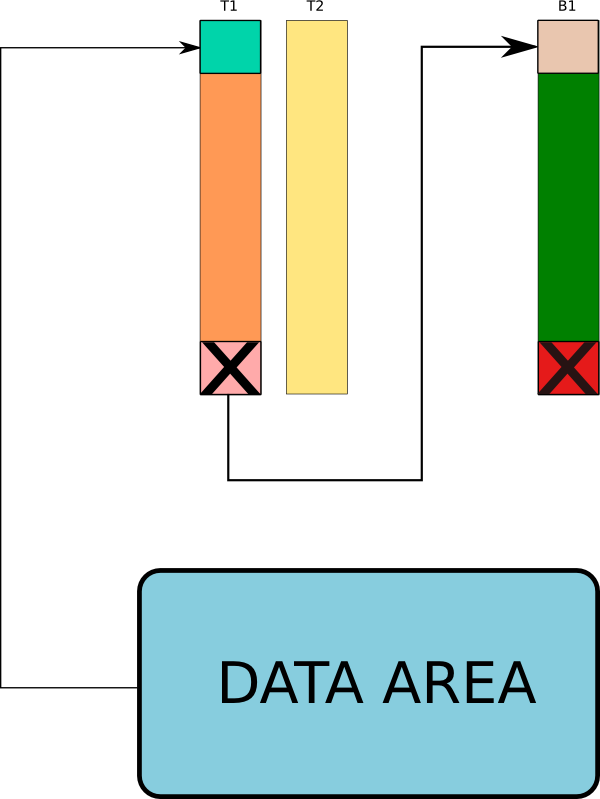
\includegraphics[scale=0.4]{images/2q_01.png}

\caption{2q, read from disk}

\end{figure}

When a backend requests a page present in T1 its CDB is removed from T1 and placed at the T2's top. The last 
element in T2 is  evicted from the shared buffer and its CDB is put at the B1's top.\newline

\begin{figure}[H]
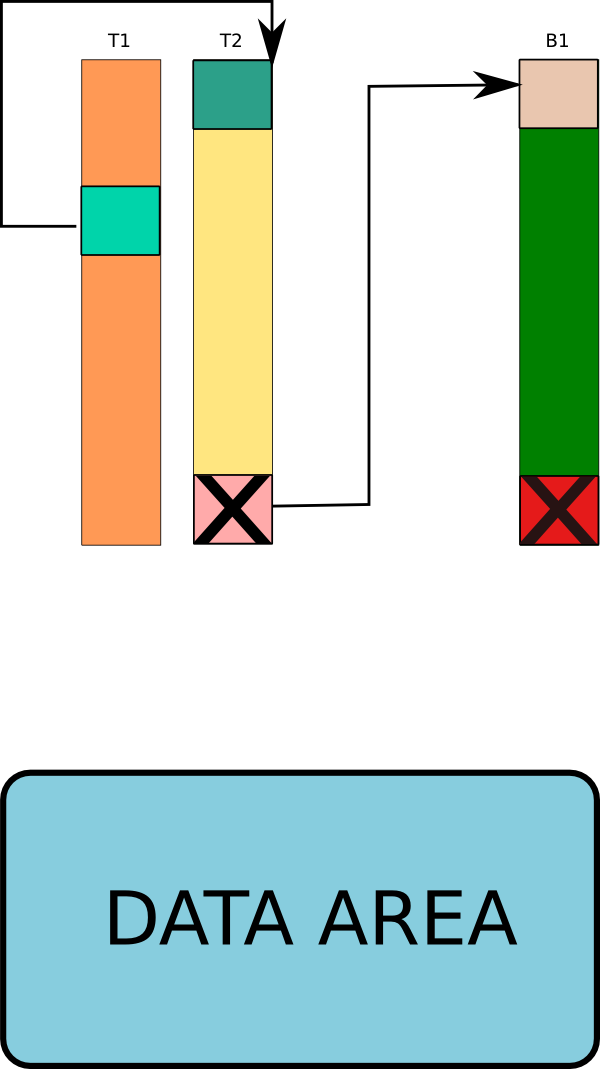
\includegraphics[scale=0.4]{images/2q_02.png}

\caption{2q, page in T1}

\end{figure}

When a backend requests a page in T2 the CDB is moved to the list's top.\newline

\begin{figure}[H]
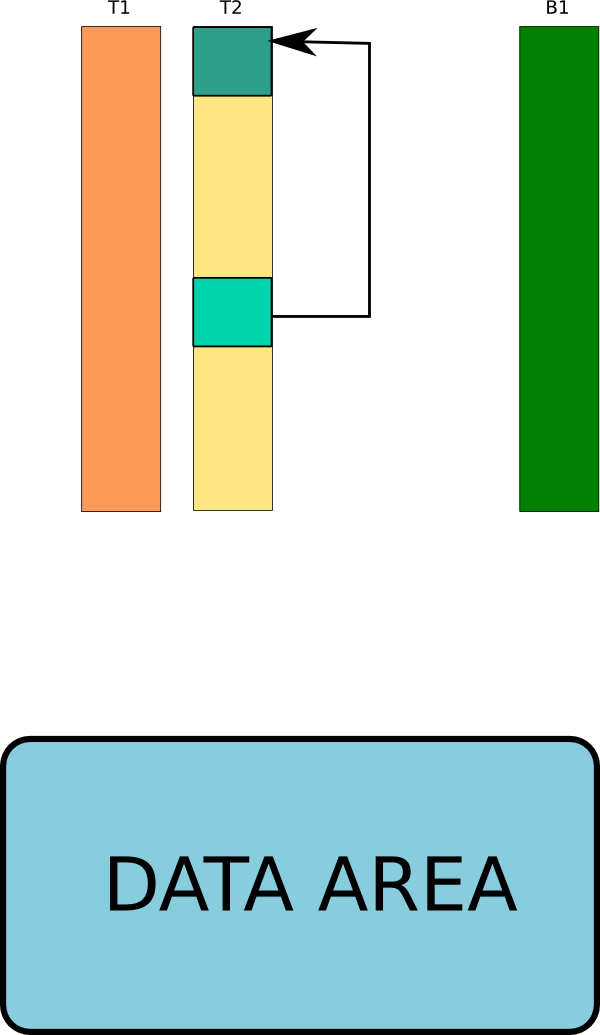
\includegraphics[scale=0.4]{images/2q_03.png}

\caption{2q, page in T2}

\end{figure}

Finally, when a page is read from the disk but its CDB is present in B1, then the page is put at the T2's 
top.\newline

\begin{figure}[H]
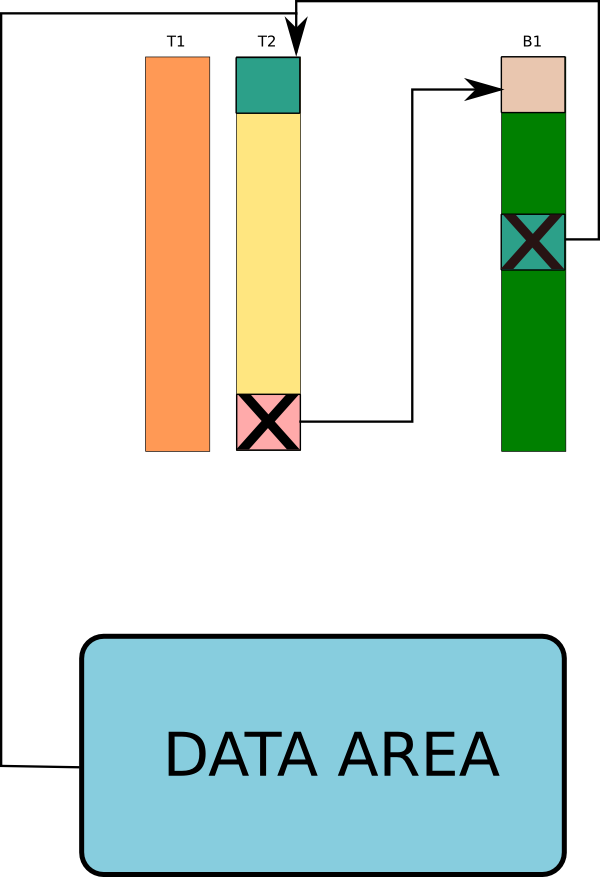
\includegraphics[scale=0.4]{images/2q_04.png}

\caption{2q, page in B1}

\end{figure}

The list T1 is the LRU list where the pages requested only one time are evicted quickly from the shared buffer. 
The list T2 is a MRU list where the pages are moved back on the top when required and where the pages from 
T1 are stored if required before the eviction. The list B1 is used as extra cache to track pages 
recently evicted from the shared buffer that need to stay in T2 if requested again.\newline

Despite the interesting approach, this tricky process did not show good performances in production. Things changed 
when the clock sweep was implemented in PostgreSQL 8.1.


\subsubsection{the ARC}
The 2q algorithm was an emergency implementation caused by a software patent held on the algorithm initially 
chosen for the PostgreSQL 8.0's memory manager. Old books, printed meanwhile the 8.0 was in development, 
wrongly list the ARC as memory manager. The ARC is an efficient algorithm which keeps in memory two 
lists of page buffers, one for the LRU and for the MRU. Each list adapts dynamically with the different requests 
of the cluster's activity. 

\subsection{PostgreSQL 8.1, the clock sweep}
The buffer manager used in PostgreSQL 8.1 was a success. Despite the algorithm simplicity offers an incredible 
flexibility adapting constantly the shared buffer's contents to the cluster's activity.\newline

The clock sweep algorithm is based on two concepts. An usage counter for the buffer and a freelist managed by a 
circular buffer. 


\subsection{PostgreSQL 8.2, the ring buffers}

\subsection{PostgreSQL 9.3, SHMMAX no more}
%todo, the change of memory allocation method happened with the 9.3

\subsection{PostgreSQL 9.4, huge pages}


\subsection{The wal buffers}

\subsection{The memory manager}
\section{The user memory}
\subsection{Work memory}
\subsection{Maintenance work memory}
\subsection{Temporary memory}


\subsection{Memory context}

\section{Wrap up}